% CANONICAL MANUSCRIPT: edit this file (GitHub or Overleaf). See docs/LATEX_OVERLEAF_AGENT_GUIDE.md.
%
% This single file is the source of truth for the IEEE midterm paper AND its supplement.
% * Edit prose freely, in GitHub or in Overleaf (main document: report/merged.tex).
% * Never edit text between "% >>> BEGIN GENERATED" and "% <<< END GENERATED" markers. Those blocks are
%   verbatim copies of report/generated/*.tex, produced from checksum-verified runs by
%   scripts/make_report_artifacts.py. Update them with: python scripts/manuscript.py sync-generated --write
% * CI compiles this file and never writes it back. Check locally: python scripts/manuscript.py check
% * Main paper = pages before \ddoptsupplement (hard limit 6 pages including references).
\documentclass[conference]{IEEEtran}
\usepackage{amsmath,amssymb}
\usepackage{graphicx}
\usepackage{booktabs}
\usepackage[numbers,sort&compress]{natbib}
\usepackage[hyphens]{url}
% URL line breaks: after punctuation, '/' or '-', never after ':' (no line ends in "https:").
\makeatletter
\def\UrlBreaks{\do\.\do\@\do\\\do\/\do\!\do\_\do\|\do\;\do\>\do\]\do\)\do\,\do\?\do\&\do\'\do+\do\=\do\#}
\def\UrlBigBreaks{\do@url@hyp}
\def\UrlNoBreaks{\do\(\do\[\do\{\do\<\do\:}
\makeatother
\usepackage[hidelinks]{hyperref}
\usepackage{needspace}
% Figures live in the repository's figures/ folder. The two paths cover compiling from report/
% (local build, CI) and from the project root (Overleaf GitHub sync) or the Overleaf ZIP.
\graphicspath{{figures/}{../figures/}}
% \runid / \repopath typeset run ids and repository paths, breakable after "/" and "_".
\newcommand{\runid}[1]{\ddoptpath{#1}}
\newcommand{\repopath}[1]{\runid{#1}}
\ExplSyntaxOn
\NewDocumentCommand{\ddoptpath}{m}{
  \group_begin: \normalfont\ttfamily
  \tl_set:Nn \l_tmpa_tl {#1}
  \tl_replace_all:Nnn \l_tmpa_tl {/} {/\allowbreak}
  \tl_replace_all:Nnn \l_tmpa_tl {\_} {\_\allowbreak}
  \tl_use:N \l_tmpa_tl
  \group_end:
}
\ExplSyntaxOff
\newcommand{\notrun}{\textbf{NOT RUN}}
\newcommand{\pending}[1]{\textbf{PENDING}\,(#1)}
% Start of the supplement: new page, S-numbered figures/tables/equations, lettered sections.
% The label supp:start marks the first supplement page; scripts/manuscript.py splits the PDF there.
\makeatletter
\newcommand{\ddoptsupplement}[1]{%
  \clearpage
  \twocolumn[{\centering{\LARGE #1\par}\vspace{0.6em}%
    {\normalsize Christian De Zabala F., Madeline Feldner, Zarar Haider, and Udaya Vijay Anand\par}%
    \vspace{1.2em}}]%
  \label{supp:start}%
  \setcounter{figure}{0}\setcounter{table}{0}\setcounter{equation}{0}%
  \renewcommand{\thefigure}{S\arabic{figure}}%
  \renewcommand{\thetable}{S\arabic{table}}%
  \renewcommand{\theequation}{S\arabic{equation}}%
  \appendices}
\makeatother
% >>> BEGIN GENERATED report/generated/status.tex (do not edit; python scripts/manuscript.py sync-generated --write)
\newcommand{\GenIsStub}{false}
\newcommand{\GenBuildNote}{Generated from the recorded runs pinned in report/runs.json}
\newcommand{\GenTestSummary}{249 passed, 0 failed, 0 errors, 1 skipped (run \runid{test\_suite\_20261027T000401Z\_2fc21cc36501}; skipped = QUA SDK not installed)}
\newcommand{\GenRunIDs}{\runid{g3\_validation\_20261026T231608Z\_cbfe38b59354}, \runid{benchmark\_scenario\_a\_20261026T232517Z\_1bd28ade742a}, \runid{benchmark\_scenario\_b\_20261026T234545Z\_ad7b16de1c23}, \runid{spectroscopy\_scenario\_a\_20261026T235246Z\_8b272601c344}, \runid{benchmark\_scenario\_a\_T4us\_20261026T235309Z\_da0c18904bc7}, \runid{convergence\_scenario\_a\_n8\_20261026T235358Z\_a8cb70bbe957}, \runid{model\_based\_scenario\_a\_20261026T235628Z\_373dfea37a30}, \runid{ablation\_colored\_20261026T235750Z\_91695709bda1}, \runid{ablation\_noamp\_20261027T000041Z\_323cd5f2b975}, \runid{ablation\_noT1\_20261027T000317Z\_20454f2f5af9}, \runid{test\_suite\_20261027T000401Z\_2fc21cc36501}}
% <<< END GENERATED report/generated/status.tex
% >>> BEGIN GENERATED report/generated/numbers.tex (do not edit; python scripts/manuscript.py sync-generated --write)
\newcommand{\AblColoredEightBothRatioHi}{0.960}
\newcommand{\AblColoredEightBothRatioLo}{0.894}
\newcommand{\AblColoredEightPhaseRatioHi}{1.004}
\newcommand{\AblColoredEightPhaseRatioLo}{1.002}
\newcommand{\AblColoredEightSel}{XY8}
\newcommand{\AblColoredEightSelEps}{2.38\times10^{-4}}
\newcommand{\AblColoredEightTimingRatioHi}{0.006}
\newcommand{\AblColoredEightTimingRatioLo}{0.006}
\newcommand{\AblColoredFourBothRatioHi}{0.986}
\newcommand{\AblColoredFourBothRatioLo}{0.967}
\newcommand{\AblColoredFourPhaseRatioHi}{1.010}
\newcommand{\AblColoredFourPhaseRatioLo}{1.006}
\newcommand{\AblColoredFourSel}{XY4}
\newcommand{\AblColoredFourSelEps}{6.31\times10^{-4}}
\newcommand{\AblColoredFourTimingRatioHi}{0.057}
\newcommand{\AblColoredFourTimingRatioLo}{0.056}
\newcommand{\AblColoredSixteenBothRatioHi}{0.566}
\newcommand{\AblColoredSixteenBothRatioLo}{0.394}
\newcommand{\AblColoredSixteenPhaseRatioHi}{0.954}
\newcommand{\AblColoredSixteenPhaseRatioLo}{0.901}
\newcommand{\AblColoredSixteenSel}{XY8}
\newcommand{\AblColoredSixteenSelEps}{9.75\times10^{-5}}
\newcommand{\AblColoredSixteenTimingRatioHi}{0.001}
\newcommand{\AblColoredSixteenTimingRatioLo}{0.001}
\newcommand{\AblNoAmpEightBothRatioHi}{1.006}
\newcommand{\AblNoAmpEightBothRatioLo}{0.992}
\newcommand{\AblNoAmpEightPhaseRatioHi}{1.009}
\newcommand{\AblNoAmpEightPhaseRatioLo}{1.007}
\newcommand{\AblNoAmpEightSel}{UDD}
\newcommand{\AblNoAmpEightSelEps}{1.02\times10^{-2}}
\newcommand{\AblNoAmpEightTimingRatioHi}{1.007}
\newcommand{\AblNoAmpEightTimingRatioLo}{0.993}
\newcommand{\AblNoAmpFourBothRatioHi}{1.018}
\newcommand{\AblNoAmpFourBothRatioLo}{0.969}
\newcommand{\AblNoAmpFourPhaseRatioHi}{1.008}
\newcommand{\AblNoAmpFourPhaseRatioLo}{0.999}
\newcommand{\AblNoAmpFourSel}{CPMG/UDD}
\newcommand{\AblNoAmpFourSelEps}{1.06\times10^{-2}/1.06\times10^{-2}}
\newcommand{\AblNoAmpFourTimingRatioHi}{1.007}
\newcommand{\AblNoAmpFourTimingRatioLo}{0.969}
\newcommand{\AblNoAmpSixteenBothRatioHi}{0.997}
\newcommand{\AblNoAmpSixteenBothRatioLo}{0.983}
\newcommand{\AblNoAmpSixteenPhaseRatioHi}{0.999}
\newcommand{\AblNoAmpSixteenPhaseRatioLo}{0.998}
\newcommand{\AblNoAmpSixteenSel}{CPMG/XY8}
\newcommand{\AblNoAmpSixteenSelEps}{1.00\times10^{-2}/1.00\times10^{-2}}
\newcommand{\AblNoAmpSixteenTimingRatioHi}{0.998}
\newcommand{\AblNoAmpSixteenTimingRatioLo}{0.987}
\newcommand{\AblNoToneEightBothRatioHi}{1.004}
\newcommand{\AblNoToneEightBothRatioLo}{0.953}
\newcommand{\AblNoToneEightPhaseRatioHi}{1.001}
\newcommand{\AblNoToneEightPhaseRatioLo}{0.996}
\newcommand{\AblNoToneEightSel}{XY8}
\newcommand{\AblNoToneEightSelEps}{3.53\times10^{-3}}
\newcommand{\AblNoToneEightTimingRatioHi}{0.081}
\newcommand{\AblNoToneEightTimingRatioLo}{0.080}
\newcommand{\AblNoToneFourBothRatioHi}{1.031}
\newcommand{\AblNoToneFourBothRatioLo}{0.917}
\newcommand{\AblNoToneFourPhaseRatioHi}{1.004}
\newcommand{\AblNoToneFourPhaseRatioLo}{1.003}
\newcommand{\AblNoToneFourSel}{XY4}
\newcommand{\AblNoToneFourSelEps}{4.00\times10^{-3}}
\newcommand{\AblNoToneFourTimingRatioHi}{0.277}
\newcommand{\AblNoToneFourTimingRatioLo}{0.271}
\newcommand{\AblNoToneSixteenBothRatioHi}{0.994}
\newcommand{\AblNoToneSixteenBothRatioLo}{0.937}
\newcommand{\AblNoToneSixteenPhaseRatioHi}{0.995}
\newcommand{\AblNoToneSixteenPhaseRatioLo}{0.991}
\newcommand{\AblNoToneSixteenSel}{XY8}
\newcommand{\AblNoToneSixteenSelEps}{3.45\times10^{-3}}
\newcommand{\AblNoToneSixteenTimingRatioHi}{0.025}
\newcommand{\AblNoToneSixteenTimingRatioLo}{0.025}
\newcommand{\BArmCMAVz}{1.01\times10^{-2}}
\newcommand{\BArmDDVz}{1.02\times10^{-2}}
\newcommand{\BArmNoDD}{2.42\times10^{-1}}
\newcommand{\BArmVzOnly}{2.88\times10^{-2}}
\newcommand{\BenchAEightBothRatioHi}{0.992}
\newcommand{\BenchAEightBothRatioLo}{0.980}
\newcommand{\BenchAEightHeadroomPct}{2.1}
\newcommand{\BenchAEightPhaseRatioHi}{1.000}
\newcommand{\BenchAEightPhaseRatioLo}{0.999}
\newcommand{\BenchAEightSel}{XY8}
\newcommand{\BenchAEightSelEps}{1.01\times10^{-2}}
\newcommand{\BenchAEightTimingRatioHi}{0.203}
\newcommand{\BenchAEightTimingRatioLo}{0.203}
\newcommand{\BenchAFourBothRatioHi}{1.011}
\newcommand{\BenchAFourBothRatioLo}{0.965}
\newcommand{\BenchAFourHeadroomPct}{6.4}
\newcommand{\BenchAFourPhaseRatioHi}{1.002}
\newcommand{\BenchAFourPhaseRatioLo}{1.001}
\newcommand{\BenchAFourSel}{XY4}
\newcommand{\BenchAFourSelEps}{1.06\times10^{-2}}
\newcommand{\BenchAFourTimingRatioHi}{0.507}
\newcommand{\BenchAFourTimingRatioLo}{0.500}
\newcommand{\BenchASixteenBothRatioHi}{0.994}
\newcommand{\BenchASixteenBothRatioLo}{0.982}
\newcommand{\BenchASixteenHeadroomPct}{1.3}
\newcommand{\BenchASixteenPhaseRatioHi}{0.998}
\newcommand{\BenchASixteenPhaseRatioLo}{0.996}
\newcommand{\BenchASixteenSel}{XY8}
\newcommand{\BenchASixteenSelEps}{1.00\times10^{-2}}
\newcommand{\BenchASixteenTimingRatioHi}{0.071}
\newcommand{\BenchASixteenTimingRatioLo}{0.071}
\newcommand{\BenchATfourEightBothRatioHi}{0.981}
\newcommand{\BenchATfourEightBothRatioLo}{0.939}
\newcommand{\BenchATfourEightPhaseRatioHi}{1.000}
\newcommand{\BenchATfourEightPhaseRatioLo}{0.999}
\newcommand{\BenchATfourEightSel}{XY8}
\newcommand{\BenchATfourEightSelEps}{2.06\times10^{-2}}
\newcommand{\BenchATfourEightTimingRatioHi}{0.352}
\newcommand{\BenchATfourEightTimingRatioLo}{0.349}
\newcommand{\BenchATfourFourBothRatioHi}{1.003}
\newcommand{\BenchATfourFourBothRatioLo}{0.975}
\newcommand{\BenchATfourFourPhaseRatioHi}{1.000}
\newcommand{\BenchATfourFourPhaseRatioLo}{1.000}
\newcommand{\BenchATfourFourSel}{XY4}
\newcommand{\BenchATfourFourSelEps}{2.28\times10^{-2}}
\newcommand{\BenchATfourFourTimingRatioHi}{0.699}
\newcommand{\BenchATfourFourTimingRatioLo}{0.693}
\newcommand{\BenchATfourSixteenBothRatioHi}{0.967}
\newcommand{\BenchATfourSixteenBothRatioLo}{0.930}
\newcommand{\BenchATfourSixteenPhaseRatioHi}{0.998}
\newcommand{\BenchATfourSixteenPhaseRatioLo}{0.997}
\newcommand{\BenchATfourSixteenSel}{XY8}
\newcommand{\BenchATfourSixteenSelEps}{1.99\times10^{-2}}
\newcommand{\BenchATfourSixteenTimingRatioHi}{0.136}
\newcommand{\BenchATfourSixteenTimingRatioLo}{0.136}
\newcommand{\BenchBEightBothCIHi}{1.032}
\newcommand{\BenchBEightBothCILo}{0.940}
\newcommand{\BenchBEightBothRatioHi}{1.004}
\newcommand{\BenchBEightBothRatioLo}{0.972}
\newcommand{\BenchBEightPhaseCIHi}{1.008}
\newcommand{\BenchBEightPhaseCILo}{0.999}
\newcommand{\BenchBEightPhaseRatioHi}{1.004}
\newcommand{\BenchBEightPhaseRatioLo}{1.002}
\newcommand{\BenchBEightTimingCIHi}{0.256}
\newcommand{\BenchBEightTimingCILo}{0.235}
\newcommand{\BenchBEightTimingRatioHi}{0.246}
\newcommand{\BenchBEightTimingRatioLo}{0.245}
\newcommand{\BenchBFourBothCIHi}{1.077}
\newcommand{\BenchBFourBothCILo}{1.004}
\newcommand{\BenchBFourBothRatioHi}{1.050}
\newcommand{\BenchBFourBothRatioLo}{1.024}
\newcommand{\BenchBFourPhaseCIHi}{1.051}
\newcommand{\BenchBFourPhaseCILo}{1.006}
\newcommand{\BenchBFourPhaseRatioHi}{1.048}
\newcommand{\BenchBFourPhaseRatioLo}{1.008}
\newcommand{\BenchBFourTimingCIHi}{0.625}
\newcommand{\BenchBFourTimingCILo}{0.553}
\newcommand{\BenchBFourTimingRatioHi}{0.612}
\newcommand{\BenchBFourTimingRatioLo}{0.568}
\newcommand{\BenchBSixteenBothCIHi}{1.016}
\newcommand{\BenchBSixteenBothCILo}{0.949}
\newcommand{\BenchBSixteenBothRatioHi}{0.993}
\newcommand{\BenchBSixteenBothRatioLo}{0.968}
\newcommand{\BenchBSixteenPhaseCIHi}{1.001}
\newcommand{\BenchBSixteenPhaseCILo}{0.994}
\newcommand{\BenchBSixteenPhaseRatioHi}{0.999}
\newcommand{\BenchBSixteenPhaseRatioLo}{0.997}
\newcommand{\BenchBSixteenTimingCIHi}{0.097}
\newcommand{\BenchBSixteenTimingCILo}{0.087}
\newcommand{\BenchBSixteenTimingRatioHi}{0.093}
\newcommand{\BenchBSixteenTimingRatioLo}{0.090}
\newcommand{\ConvBestBaselineTrain}{1.08\times10^{-2}}
\newcommand{\ConvBestBaselineVal}{1.03\times10^{-2}}
\newcommand{\ConvTimingXYTrainFinal}{8.87\times10^{-3}}
\newcommand{\ConvTimingXYValFinal}{1.03\times10^{-2}}
\newcommand{\ConvTrainFinal}{9.37\times10^{-3}}
\newcommand{\ConvValFinal}{1.03\times10^{-2}}
\newcommand{\FloorA}{9.90\times10^{-3}}
\newcommand{\GthreeMaxZ}{0.95}
\newcommand{\GthreeNtraj}{64000}
\newcommand{\GthreeRelSEHi}{0.56}
\newcommand{\GthreeRelSELo}{0.52}
\newcommand{\MBFitFullEightRatioHi}{0.991}
\newcommand{\MBFitFullEightRatioLo}{0.966}
\newcommand{\MBFitFullFourRatioHi}{1.011}
\newcommand{\MBFitFullFourRatioLo}{0.982}
\newcommand{\MBFitRedEightRatioHi}{0.986}
\newcommand{\MBFitRedEightRatioLo}{0.896}
\newcommand{\MBFitRedFourRatioHi}{0.984}
\newcommand{\MBFitRedFourRatioLo}{0.894}
\newcommand{\MBTruthEightRatioHi}{0.992}
\newcommand{\MBTruthEightRatioLo}{0.980}
\newcommand{\MBTruthFourRatioHi}{1.011}
\newcommand{\MBTruthFourRatioLo}{0.965}
\newcommand{\PinnedRunsDirty}{5}
\newcommand{\PinnedRunsDirtyList}{pre-registered spectroscopy (G4) run, pre-registered $T=4\,\mu$s benchmark, no-amplitude-error ablation, no-$T_1$ ablation, and historical test-suite record}
\newcommand{\PinnedRunsTotal}{11}
\newcommand{\RobBEightBothWinsMax}{9}
\newcommand{\RobBEightBothWinsMin}{0}
\newcommand{\RobBEightBothWorstMax}{2.08\times10^{-2}}
\newcommand{\RobBEightDDWorst}{1.02\times10^{-2}}
\newcommand{\RobBEightPhaseWinsMax}{8}
\newcommand{\RobBEightPhaseWinsMin}{7}
\newcommand{\RobBEightPhaseWorstMax}{1.05\times10^{-2}}
\newcommand{\RobBEightVzBest}{2.88\times10^{-2}}
\newcommand{\RobBEightVzWorst}{3.86\times10^{-2}}
\newcommand{\RobBFourBothWinsMax}{8}
\newcommand{\RobBFourBothWinsMin}{3}
\newcommand{\RobBFourBothWorstMax}{2.11\times10^{-2}}
\newcommand{\RobBFourDDWorst}{1.13\times10^{-2}}
\newcommand{\RobBFourPhaseWinsMax}{10}
\newcommand{\RobBFourPhaseWinsMin}{10}
\newcommand{\RobBFourPhaseWorstMax}{1.12\times10^{-2}}
\newcommand{\RobBFourVzBest}{2.88\times10^{-2}}
\newcommand{\RobBFourVzWorst}{3.86\times10^{-2}}
\newcommand{\RobBSixteenBothWinsMax}{0}
\newcommand{\RobBSixteenBothWinsMin}{0}
\newcommand{\RobBSixteenBothWorstMax}{1.50\times10^{-2}}
\newcommand{\RobBSixteenDDWorst}{1.00\times10^{-2}}
\newcommand{\RobBSixteenPhaseWinsMax}{0}
\newcommand{\RobBSixteenPhaseWinsMin}{0}
\newcommand{\RobBSixteenPhaseWorstMax}{1.04\times10^{-2}}
\newcommand{\RobBSixteenVzBest}{2.88\times10^{-2}}
\newcommand{\RobBSixteenVzWorst}{3.86\times10^{-2}}
\newcommand{\SpecGaussFullAfCov}{0.934}
\newcommand{\SpecGaussFullAfRmseRatio}{1.15}
\newcommand{\SpecGaussFullCov}{0.934}
\newcommand{\SpecGaussFullRmseRatio}{1.15}
\newcommand{\SpecGaussRedCov}{0.877}
\newcommand{\SpecGaussRedRmseRatio}{1.26}
\newcommand{\SpecTelFullCov}{0.962}
\newcommand{\SpecTelFullRmseRatio}{1.05}
\newcommand{\SpecTelRedCov}{0.934}
\newcommand{\SpecTelRedRmseRatio}{1.16}
\newcommand{\SpecTruthTtwoHahn}{28.08}
\newcommand{\SpecTruthTtwoStar}{9.14}
\newcommand{\TestsPassed}{249}
% <<< END GENERATED report/generated/numbers.tex
\IEEEspecialpapernotice{Midterm Report, October 27, 2026}
% 2+2 author layout (IEEEtran puts all \and-separated blocks on one row otherwise).
\makeatletter
\newcommand{\linebreakand}{\end{@IEEEauthorhalign}\hfill\mbox{}\par\mbox{}\hfill\begin{@IEEEauthorhalign}}
\makeatother
\title{Model-Based Dynamical Decoupling for Idle Superconducting Qubits\\
\large A Reproducible Synthetic Benchmark with Hardware Timing Constraints}
\author{
\IEEEauthorblockN{Christian De Zabala F.}
\IEEEauthorblockA{Department of Computer Science\\Department of Economics\\Columbia University\\cd3441@columbia.edu}
\and
\IEEEauthorblockN{Madeline Feldner}
\IEEEauthorblockA{Department of Computer Science\\Department of Statistics\\Columbia University\\mef2238@columbia.edu}
\linebreakand
\IEEEauthorblockN{Zarar Haider}
\IEEEauthorblockA{Department of Computer Science\\Columbia University\\zh2555@columbia.edu}
\and
\IEEEauthorblockN{Udaya Vijay Anand}
\IEEEauthorblockA{Department of Electrical Engineering\\Columbia University\\uv2125@columbia.edu}
}
\begin{document}
\maketitle
\begin{abstract}
An idle superconducting qubit that waits during a neighbour's mid-circuit measurement loses
coherence to stochastic dephasing and to deterministic frequency shifts. We ask whether optimizing
dynamical-decoupling (DD) pulse timings and phases against a noise model with the covariance matrix
adaptation evolution strategy (CMA-ES) outperforms strong canonical sequences. We pre-registered a
synthetic transmon-like model, seeds, baselines and a training-only baseline-selection rule, and scored
every arm on independent held-out noise. A finite-pulse Monte Carlo simulator agrees with
filter-function theory in five predetermined configurations (largest $|z|=\GthreeMaxZ$), and synthetic
spectroscopy yields a predictive but not uniquely identified noise model (held-out RMSE
$\SpecGaussFullRmseRatio\times$ the shot-noise floor). In the pre-registered Scenario~A, the selected
XY4/XY8 baselines lie within $\BenchASixteenHeadroomPct$--$\BenchAFourHeadroomPct\%$ of the
relaxation-plus-white-noise floor, which bounds any possible gain; no CMA-ES mode improved on them by
more than about 1\%. With a deterministic Stark-like shift and virtual-$Z$ correction, CMA-ES gained a
few percent only at $n=4$, and the timing+phase gain did not survive $\pm100$\,ns readout-timing
shifts. Exploratory colored-noise ablations with more headroom also showed no substantial held-out
gain. All results are synthetic; no quantum hardware was used.
\end{abstract}
\begin{IEEEkeywords}
dynamical decoupling, superconducting qubits, noise spectroscopy,
CMA-ES, synthetic simulation, quantum control
\end{IEEEkeywords}

\section{Introduction}
\label{sec:intro}
An idle spectator qubit must preserve coherence while other qubits are measured and classical
feedback is processed. It accumulates phase errors from stochastic dephasing and, in dynamic
circuits, from deterministic frequency shifts during neighbouring readout. Dynamical decoupling
suppresses suitable low-frequency dephasing, but finite pulse errors, energy relaxation ($T_1$) and
broadband fluctuations limit the achievable improvement. We investigate whether model-based
optimization of DD sequences reduces idle-window infidelity relative to strong canonical sequences
under a fixed pulse budget and identical constraints, and we report how much improvement the model
permits in the first place.

\paragraph{Research questions}
\begin{description}
  \item[RQ1] Does Monte Carlo coherence agree with analytic filter-function predictions under matched
    power-spectral-density (PSD) conventions?
  \item[RQ2] How accurately do noise models fitted to synthetic Ramsey, Hahn and
    Carr--Purcell--Meiboom--Gill (CPMG) data predict held-out decays?
  \item[RQ3] Does joint optimization of pulse timings and phases beat strong DD baselines on held-out
    noise in Scenario~A (stochastic dephasing)?
  \item[RQ4] Does any gain over calibrated virtual-$Z$ correction plus standard DD survive uncertainty in
    a readout-induced detuning (Scenario~B)?
  \item[RQ5] How robust are the results to pulse imperfections and model mismatch?
\end{description}

\paragraph{Scope} This is a synthetic computational study; validation on superconducting hardware is
a separate, planned experiment. Scenarios, seeds, baselines, the baseline-selection rule and the
metric (average gate infidelity against the frame-corrected target, Sec.~\ref{sec:model}) were
pre-registered in the repository before any optimization run, and deviations are logged. A zero gain
or a regression counts as a valid outcome.

\section{Related work}
\label{sec:related}
Dynamical decoupling of open quantum systems was introduced by \citet{Viola1999}.
\citet{Uhrig2007} proposed optimized $\pi$-pulse sequences, and \citet{Cywinski2008} analysed how to
enhance dephasing times in superconducting qubits. \citet{Biercuk2009} studied optimized DD in a
model quantum memory. DD design has been cast as a filter-design problem
\citep{BiercukDohertyUys2011}, and higher-order filtering has been developed for nontrivial gates
\citep{GreenUysBiercuk2012}; these deterministic, filter-function objectives differ from the
finite-trajectory Monte Carlo objective used here. DD has also served as a noise spectrometer, with a
superconducting flux qubit \citep{Bylander2011} and for colored noise in general \citep{Alvarez2011}.
Robust DD sequences were studied by \citet{Souza2011}, and \citet{Ezzell2023} surveyed DD performance
on superconducting qubits.

Learning-based approaches tailor DD to hardware empirically: \citet{Rahman2024} optimize the rotational
gates of DD sequences for superconducting hardware, \citet{Tong2025} learn DD empirically on quantum
processors, and \citet{Tong2026} study learned error suppression in dynamic circuits. Our approach
instead optimizes against a fitted or assumed noise model. This avoids hardware calls during the search
but depends on model fidelity. Our contribution is limited to a pre-registered, held-out synthetic
benchmark of model-based DD optimization with explicit noise floors; it does not test transfer to
hardware.

\section{Physical model and conventions}
\label{sec:model}
We use $\hbar=1$, time in s, angular frequency and detuning in rad/s, and angles in rad. In the
rotating frame of the drive,
\begin{multline}
  H(t) = \tfrac{1}{2}\bigl[\delta(t) + d(t) + \delta_{\mathrm{off}}\bigr]\sigma_z\\
       + \tfrac{1}{2}\Omega(t)\bigl[\cos\varphi(t)\,\sigma_x + \sin\varphi(t)\,\sigma_y\bigr],
\end{multline}
where $\delta(t)$ is zero-mean stationary noise, assumed Gaussian unless stated otherwise, $d(t)$ is a
known deterministic detuning profile (e.g.\ during neighbouring readout), and $\delta_{\mathrm{off}}$ is
a static calibration offset.

\paragraph{Spectrum and filter} With autocorrelation $C(\tau)=\langle\delta(t+\tau)\delta(t)\rangle$
we use the two-sided PSD $S_2(\omega)=\int_{-\infty}^{\infty} C(\tau)e^{-i\omega\tau}\,d\tau$ in
rad$^2$/s. For the switching function $y(t)$ (toggling-frame $z$ component, $\pm1$ between ideal
$\pi$ pulses),
\begin{gather}
  Y(\omega)=\int_0^T y(t)e^{i\omega t}\,dt,\\
  \chi=\operatorname{Var}\phi=\frac{1}{2\pi}\int_{-\infty}^{\infty} S_2(\omega)\,|Y(\omega)|^2\,d\omega,
\end{gather}
and, under the Gaussian assumption, the coherence is $W=e^{-\chi/2}$ with pure-dephasing average gate
infidelity $r=(1-W)/3$. Low- and high-frequency cutoffs of $S_2$ are stated for every model.

\paragraph{Energy relaxation} $T_1$ is modelled as amplitude damping with $\gamma=1-e^{-t/T_1}$ per
free segment. Channels are composed as Pauli transfer matrices (PTMs), never by adding infidelities.
Amplitude damping alone has average infidelity $r_{\rm AD}=(2+\gamma-2\sqrt{1-\gamma})/6\approx\gamma/3$.

\paragraph{Target and frame correction} Fidelity is evaluated against
$U_{\mathrm{target}}=R_z(\theta_{\mathrm{vz}})U_0$, where $U_0$ is the ideal net control unitary of the
sequence and $\theta_{\mathrm{vz}}$ a virtual-$Z$ correction of the known $d(t)$ (zero unless frame
correction is allowed). A channel with PTM $R$ has average gate fidelity
$F_{\mathrm{avg}}=(\operatorname{Tr}R'+2)/6$ with $R'=R_{\mathrm{target}}^{\mathsf T}R$. For finite
pulses the generalized (three-component) filter function makes $W=e^{-\chi/2}$ leading-order only; the
Monte Carlo simulator needs neither approximation. Finite pulse widths, minimum spacing and the timing
grid are enforced for all sequences.

\section{Methods}
\label{sec:methods}
\paragraph{Synthetic device (Scenario~A)} All device numbers are assumptions, fixed in a pre-registered
plan (\repopath{docs/EXPERIMENT\_PLAN.md}). The idle window is $T=2\,\mu$s (alternate $4\,\mu$s), with
square $\pi$ pulses of width $w=32$\,ns, a 4\,ns guard and pulse starts on a 4\,ns grid (an assumed
controller tick). The dephasing PSD sums a band-limited $1/f$ term ($2\pi\cdot1$\,Hz to
$2\pi\cdot10$\,MHz, $S_2=A/|\omega|$, $A=5.929\times10^9$, calibrated to an isolated Ramsey coherence of
$e^{-1}$ at $10\,\mu$s), a Gaussian Ornstein--Uhlenbeck (Lorentzian) term with
$\sigma=1.236\times10^5$\,rad/s and $\tau_c=0.5\,\mu$s, and a white floor $S_0=10^4$\,rad$^2$/s;
$T_1=100\,\mu$s, and each trajectory draws a relative Rabi-amplitude error
$\epsilon_\Omega\sim\mathcal N(0,0.02^2)$. Scenario~B adds a deterministic Stark-like shift of
$2\pi\cdot0.2$\,MHz between 0.6 and 1.6\,$\mu$s (20\,ns tanh edges) as a stand-in for a neighbouring
readout. It models a known frequency shift only, not measurement-induced dephasing.

\paragraph{Finite-pulse simulator} Gaussian noise trajectories are sampled on a 1\,ns grid by hybrid
spectral synthesis (long periodic FFT plus explicit low-frequency random-phase quadrature; exact
recursions for the Lorentzian and for telegraph noise). Free segments are exact $z$ rotations; pulses
are propagated in 8 piecewise-constant sub-steps including detuning. Amplitude damping is composed per
free segment and approximated as $\mathrm{AD}(w/2)\,U\,\mathrm{AD}(w/2)$ during pulses. The reported
$\epsilon$ is the mean per-trajectory infidelity, which equals the channel infidelity because
$F_{\rm avg}$ is linear in the channel. Unit tests check unitarity, zero-noise compensated infidelity
($\le10^{-10}$ for all families), second-order convergence in time step and pulse sub-steps, and the
$T_1$-only formula.

\paragraph{Spectroscopy} Synthetic Ramsey, Hahn, CPMG-2 and CPMG-4 data (14 log-spaced idle times in
$[0.1,40]\,\mu$s, 1000 shots per point, binomial shot noise, an affine state-preparation-and-measurement
map) are fitted by binomial maximum likelihood with a parametric bootstrap. A \emph{reduced} Gaussian
model ($1/f$ plus white) and a \emph{full} model (plus Lorentzian) are fitted with $T_1$ treated as known,
because white dephasing and $1/T_1$ are degenerate for instantaneous pulses. Held-out data (CPMG-8,
CPMG-16, and the training families at 13 unseen times) are drawn with an independent generator and
never seen by the fit.

\paragraph{Optimizer and training objective} We use pycma 4.5.0 \citep{Hansen2016}, an evolution
strategy (not reinforcement learning). Timings are encoded by $n$ unconstrained coordinates through a
softmax over the free time with a minimum gap, snapped to the grid; unrepairable candidates are
rejected. Phase offsets are projected so that the ideal net unitary equals the base sequence's, so
fidelity is never graded against the wrong target. Three modes are run, timing-only, phase-only and
timing+phase, all initialized at CPMG timing with $Y$ pulse axes. The objective is the mean infidelity
over a fixed set of 256 frozen training trajectories (common random numbers), with a budget of 2000
evaluations and three independent training runs (training seeds 101--103, optimizer seeds 1--3).
A frozen finite sample makes the objective a noisy surrogate of the expected infidelity: differences
between candidates below its sampling error can be selected by chance, and the search can fit the
particular trajectories. We did not vary the number of training trajectories or the budget, so these
effects are not separated from the parameterization. A deterministic filter-function objective is a
natural alternative but was \emph{not} used in this benchmark.

\paragraph{Baselines and evaluation} At each pulse number $n$ the baselines are CPMG-$n$ ($Y$ pulses),
XY4, XY8 (where $n$ divides), Uhrig DD (UDD-$n$) and free evolution, all with the same $T$, $w$, guard,
grid, noise model and frame-correction privileges. The pre-registered rule selects the baseline with the
lowest \emph{training} infidelity. All arms are then evaluated on the same held-out draws (seeds
9001--9005, 1024 trajectories each; disjointness from training is enforced in code). We report raw
$\epsilon$, the ratio $\epsilon_{\rm sel}/\epsilon_{\rm CMA}$ ($>1$ favours CMA-ES), and a two-stage
paired-bootstrap 95\% interval (seeds as blocks). These intervals quantify Monte Carlo uncertainty within
the synthetic model only; they are not significance tests and do not account for model selection or
mismatch. The timing-only arm keeps CPMG's $Y$ axes, so it compares retimed CPMG with XY4/XY8 and
conflates timing with the choice of phases (Sec.~\ref{sec:results}).

\paragraph{Reproducibility} Each run writes an immutable \repopath{results/<run\_id>/} directory with a
manifest (time, git commit and dirty flag, platform, package versions, configuration hash, seeds,
command) and SHA-256 checksums. Every number, table and figure here is regenerated by
\repopath{scripts/make\_report\_artifacts.py} from runs pinned in \repopath{report/runs.json}; the
claim-to-artifact ledger is \repopath{report/evidence\_map.csv}. The historical full test suite
recorded \GenTestSummary; continuous integration reruns the smoke tests on every commit.

\section{Experimental results}
\label{sec:results}
All results are simulation predictions for the synthetic model of Sec.~\ref{sec:methods}; detailed
tables and diagnostics are in the supplement (Tables~\ref{tab:g3}--\ref{tab:feasibility},
Figs.~\ref{fig:bench}--\ref{fig:rob}).

\subsection{Simulator and spectroscopy validation (RQ1, RQ2)}
In five predetermined configurations, Monte Carlo infidelity agrees with the ideal filter-function
reference within the combined uncertainty (largest standardized discrepancy $|z|=\GthreeMaxZ$,
Table~\ref{tab:g3}). This establishes internal consistency of two implementations of the same model,
not device validation. The full Gaussian fit predicts 106 held-out decay points (Fig.~\ref{fig:spec})
with RMSE $\SpecGaussFullRmseRatio\times$ the shot-noise floor and 95\% predictive coverage
$\SpecGaussFullCov$. This is a favourable test: the data come from the same analytic forward family
that is fitted, with $T_1$ and the $1/f$ cutoffs fixed at their true values and a single data seed.
The spectrum itself is not uniquely identified: the Lorentzian parameters are strongly correlated, the
band above $\sim$1\,MHz is barely constrained, and only the derived decay predictions are well
determined.

\begin{figure}[t]
\centering
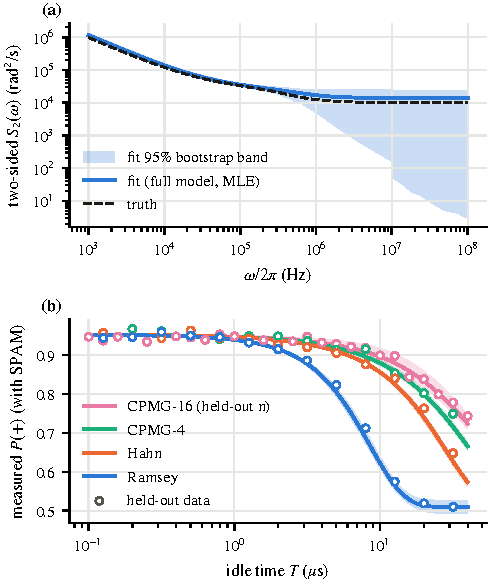
\includegraphics[width=\linewidth]{fig_spectroscopy.pdf}
\caption{Synthetic noise spectroscopy (full Gaussian model). (a) True and fitted two-sided PSD with a
95\% parametric-bootstrap band; the spectrum is weakly constrained outside the sampled passbands.
(b) Fitted decay curves with 95\% bands; open circles are independent held-out points only.}
\label{fig:spec}
\end{figure}

\subsection{Scenario A: canonical DD versus optimization (RQ3)}
Table~\ref{tab:main} and Fig.~\ref{fig:benchratio} summarize the pre-registered held-out comparison.
The training-only rule selects XY4 at $n=4$ and XY8 at $n=8,16$. The largest ratio is
$\BenchAFourBothRatioHi$ (one $n=4$ timing+phase run), a gain of about 1\% whose interval includes 1;
phase-only ratios lie within $\pm0.4\%$ of 1, and timing+phase is otherwise neutral or worse.

The model leaves little room for any optimizer. XY8 reaches $\epsilon=\BenchASixteenSelEps$ at $n=16$,
against a pulse-independent floor of $\FloorA$ set by $T_1$ and white dephasing (which ideal refocusing
does not suppress). An optimizer that removed every decouplable error would therefore reduce infidelity
by at most $\BenchASixteenHeadroomPct\%$ at $n=16$ and $\BenchAFourHeadroomPct\%$ at $n=4$
(Table~\ref{tab:main}). The Scenario~A null result is thus a statement about this model's headroom as
much as about the optimizer, and it does not show that CMA-ES is ineffective for DD in general.

The timing-only arm (ratios $\BenchASixteenTimingRatioLo$--$\BenchAFourTimingRatioHi$) fails for a
different reason: it keeps CPMG's $Y$ axes, and CPMG accumulates the 2\% amplitude error that XY-type
phase cycling cancels. It therefore measures retimed CPMG against XY4/XY8, not the value of timing
optimization. In one exploratory run that optimized timings with XY8 phases fixed
(Fig.~\ref{fig:conv}), validation infidelity reached $\ConvTimingXYValFinal$, equal to XY8
($\ConvBestBaselineVal$) at this precision. In both that run and the timing+phase run, training
infidelity fell well below XY8's ($\ConvTimingXYTrainFinal$ and $\ConvTrainFinal$ versus
$\ConvBestBaselineTrain$) without any validation gain, consistent with fitting the 256 frozen
trajectories.

% >>> BEGIN GENERATED report/generated/main_table.tex (do not edit; python scripts/manuscript.py sync-generated --write)
\begin{table}[t]
\centering\scriptsize\setlength{\tabcolsep}{3pt}
\caption{Held-out summary at $T=2\,\mu$s (test seeds 9001--9005). Sel.: baseline chosen by the
pre-registered training-only rule; $\epsilon_{\rm sel}$ in units of $10^{-3}$. Headroom: largest possible
relative reduction $1-\epsilon_{\rm floor}/\epsilon_{\rm sel}$ (\%) if the $T_1$-plus-white-noise floor were
reached. Ratio $\epsilon_{\rm sel}/\epsilon_{\rm CMA}$ ranges over 3 training runs ($>1$ favours CMA-ES).
Scenario~B arms use virtual-$Z$. Runs: \runid{benchmark\_scenario\_a\_20261026T232517Z\_1bd28ade742a}; \runid{benchmark\_scenario\_b\_20261026T234545Z\_ad7b16de1c23}.}
\label{tab:main}
\resizebox{\columnwidth}{!}{\begin{tabular}{@{}cccccccc@{}}\toprule
Scen. & $n$ & Sel. & $\epsilon_{\rm sel}$ & Headroom & timing-only & phase-only & timing+phase\\\midrule
A & 4 & XY4 & 10.6 & 6.4 & 0.500--0.507 & 1.001--1.002 & 0.965--1.011 \\
 & 8 & XY8 & 10.1 & 2.1 & 0.203--0.203 & 0.999--1.000 & 0.980--0.992 \\
 & 16 & XY8 & 10.0 & 1.3 & 0.071--0.071 & 0.996--0.998 & 0.982--0.994 \\
\addlinespace
B & 4 & XY4 & 11.1 & 10.6 & 0.568--0.612 & 1.008--1.048 & 1.024--1.050 \\
 & 8 & XY4 & 10.2 & 2.5 & 0.245--0.246 & 1.002--1.004 & 0.972--1.004 \\
 & 16 & XY8 & 10.0 & 1.3 & 0.090--0.093 & 0.997--0.999 & 0.968--0.993 \\
\bottomrule\end{tabular}}\end{table}
% <<< END GENERATED report/generated/main_table.tex

\begin{figure}[t]
\centering
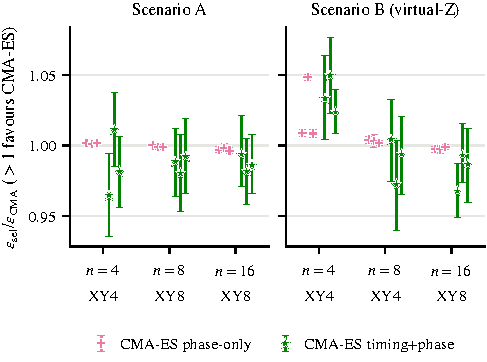
\includegraphics[width=\linewidth]{fig_benchmark_ratio.pdf}
\caption{Held-out ratio $\epsilon_{\rm sel}/\epsilon_{\rm CMA}$ ($>1$ favours CMA-ES) for each of three
training runs, at the same $n$ and $T=2\,\mu$s as the training-selected baseline named under each $n$.
Bars: pooled paired-bootstrap 95\% intervals (Monte Carlo uncertainty within the model only).
Timing-only CMA-ES (ratios $\BenchASixteenTimingRatioLo$--$\BenchBFourTimingRatioHi$) is omitted for
clarity; see Table~\ref{tab:main}.}
\label{fig:benchratio}
\end{figure}

\subsection{Scenario B: readout-like detuning (RQ4)}
Scenario~B adds a known, deterministic Stark-like frequency profile; it does not model stochastic
measurement-induced dephasing or measured readout. At $n=8$ the four pre-registered arms reach
$\epsilon=\BArmNoDD$ (no DD, no frame correction), $\BArmVzOnly$ (virtual-$Z$ only), $\BArmDDVz$ (best
canonical DD plus virtual-$Z$) and $\BArmCMAVz$ (CMA-ES plus virtual-$Z$), so most of the benefit comes
from frame correction combined with any XY-type sequence. At the nominal profile CMA-ES beats
XY4 plus virtual-$Z$ only at $n=4$, by ratios $\BenchBFourPhaseRatioLo$--$\BenchBFourPhaseRatioHi$
(phase-only) and $\BenchBFourBothRatioLo$--$\BenchBFourBothRatioHi$ (timing+phase). The pre-registered
robustness sweep reverses the timing+phase gain: under $\pm50$--$100$\,ns readout-timing shifts its
worst case reaches $\RobBFourBothWorstMax$ against $\RobBFourDDWorst$ for XY4 plus virtual-$Z$
(Table~\ref{tab:robustness}, Fig.~\ref{fig:rob}). Only the $n=4$ phase-only sequences stay marginally
better in all ten perturbed profiles. These $n=4$ cells were singled out after inspecting about 27
Scenario~B comparisons and are exploratory.

\subsection{Ablations and model mismatch (RQ5)}
The exploratory ablations, added after the pre-registered results and evaluated on the same test seeds,
probe whether headroom changes the conclusion. Removing $T_1$ and the white floor (``colored only'')
lowers XY8's infidelity to $\AblColoredSixteenSelEps$ at $n=16$, two orders of magnitude of headroom.
Even so, within the same 2000-evaluation budget CMA-ES gained at most 0.4\% over XY8 at $n=8$ (ratios
up to $\AblColoredEightPhaseRatioHi$) and timing+phase lost substantially at $n=16$ (ratio
$\AblColoredSixteenBothRatioLo$--$\AblColoredSixteenBothRatioHi$; Table~\ref{tab:ablation}). Optimizing
on a model \emph{fitted} from synthetic spectroscopy and testing on the truth gives ratios
$\MBFitFullFourRatioLo$--$\MBFitFullFourRatioHi$ at $n=4$ (Table~\ref{tab:model_based}), so
identification error adds loss.

\section{Discussion and limitations}
\label{sec:discussion}
\paragraph{Interpretation} Under the pre-registered model the answer to RQ3 is negative, but the test
had limited discriminatory power: XY4/XY8 already suppress the decouplable colored noise, and the
remaining infidelity is set by $T_1$ and white dephasing. The headroom in Table~\ref{tab:main} should be
computed before any search. Where headroom exists (the colored-only ablation), our configuration still
did not generalize better than XY-family designs. Training gains on frozen trajectories, the timing-only
arm's CPMG phases, and a search that starts from CPMG rather than XY8 are all plausible contributors.
These are statements about this parameterization, budget and synthetic model, not about CMA-ES or
learned DD in general. The one positive signal (Scenario~B, $n=4$) is a few percent, was identified
after the fact, and would need a new pre-registered test.

\paragraph{Limitations}
\begin{itemize}
  \item All evidence is synthetic: device parameters are assumptions, and optimizing against the model
    used for evaluation is circular. Spectroscopy data share the fitted model's analytic form.
  \item Noise is Gaussian and stationary (the telegraph control is nearly Gaussian at our parameters).
    Scenario~B is a known frequency shift; measurement-induced dephasing is not modelled.
  \item $T_1$ during pulses is approximated; leakage, crosstalk, finite bandwidth and pulse shaping are
    absent, and pulse errors are a static per-trajectory amplitude error.
  \item Intervals capture Monte Carlo sampling only; five test seeds resolve seed-level variability
    coarsely. The ablations and convergence diagnostic are exploratory and reused the test seeds, and
    robustness to drift, Stark rise time and grid quantization was not evaluated.
  \item $\PinnedRunsDirty$ of the $\PinnedRunsTotal$ pinned runs recorded a dirty working tree
    without the uncommitted diff: the \PinnedRunsDirtyList. Their checksums prove the stored files are
    unchanged, not which code produced them; the manifests are preserved as recorded, and a later clean
    rerun would not establish the historical code either.
  \item No hardware was used. The QUA (Quantum Machines) adapter is a schedule translator marked
    \emph{not hardware tested}. Bibliographic identities were checked against arXiv; remaining
    publisher metadata checks are listed in \repopath{docs/CITATION\_AUDIT.md}.
\end{itemize}

\paragraph{Roadmap} (i) With authorization, measure $T_1$, Ramsey, Hahn and CPMG decays and spectator
phase during neighbour readout on the target device, to establish whether the decouplable colored
component is large enough for optimization to matter. (ii) Model measurement-induced dephasing as
non-stationary noise and repeat Scenario~B. (iii) Pre-register a new benchmark with an analytic
filter-function or larger-sample objective, an XY8 starting point and timing-only arms with XY phases.

\section*{Author contributions}
Christian De Zabala F., Madeline Feldner, Zarar Haider, and Udaya Vijay Anand contributed equally to
this project, including its research, implementation, evaluation, and report preparation.

{\raggedright\footnotesize\noindent\textbf{Code, data and supplement:}
\url{https://github.com/udsy19/quantum-dd-optimizer}; project website
\url{https://udsy19.github.io/quantum-dd-optimizer/}.\par}

\bibliographystyle{IEEEtranN}
\IfFileExists{refs.bib}{\bibliography{refs}}{\bibliography{report/refs}}

% =====================================================================================================
% SUPPLEMENT (does not count toward the 6-page main-paper limit). Figures, tables and equations are
% numbered S1, S2, ...; citations refer to the reference list of the main paper.
% =====================================================================================================
\ddoptsupplement{Supplementary Material: Detailed Synthetic Results}

\noindent This supplement extends Sec.~\ref{sec:results} of the main paper with full tables, run
identifiers and diagnostics. All numbers are simulation predictions for the synthetic model of
Sec.~\ref{sec:methods}, generated from the recorded runs listed in Appendix~\ref{supp:prov}; none is a
measurement. Citations refer to the main paper's reference list.

\section{Simulator validation (RQ1)}
\label{supp:g3}
Table~\ref{tab:g3} lists five predetermined configurations: free evolution, Hahn and CPMG-8, the last
two with both 32\,ns and instantaneous pulses. In every configuration the finite-pulse Monte Carlo
infidelity agrees with the analytic prediction within $1.96$ standard errors ($\GthreeNtraj$
trajectories per case; largest $|z|=\GthreeMaxZ$), and halving the noise time step changes each
estimate by less than the combined statistical error. The PSD normalization, filter function, noise
sampler and propagator are therefore mutually consistent at the resolution of this test (standard
errors of $\GthreeRelSELo$--$\GthreeRelSEHi\%$ of $r$).

% >>> BEGIN GENERATED report/generated/g3_table.tex (do not edit; python scripts/manuscript.py sync-generated --write)
\begin{table}[t]
\centering\scriptsize\setlength{\tabcolsep}{3pt}
\caption{Gate G3: Monte-Carlo (finite-pulse simulator, 64000 noise trajectories per row, $dt=1$\,ns)
versus filter-function prediction $r=(1-e^{-\chi/2})/3$, Scenario~A Gaussian noise without $T_1$ or
control errors, $T=2\,\mu$s. Pass criterion: $|r_{\rm MC}-r_{\rm FF}|\le1.96\,\mathrm{SE}+$quadrature error.
Run \runid{g3\_validation\_20261026T231608Z\_cbfe38b59354}.}
\label{tab:g3}
\resizebox{\columnwidth}{!}{\begin{tabular}{@{}lcccc@{}}\toprule
Configuration & $10^3 r_{\rm FF}$ & $10^3 r_{\rm MC}\pm$SE & $z$ & Pass\\\midrule
Free (Ramsey) & 21.785 & 21.673$\pm$0.117 & $-0.95$ & yes \\
Hahn, $w=32$\,ns & 6.087 & 6.093$\pm$0.033 & $+0.18$ & yes \\
CPMG-8, $w=32$\,ns & 3.548 & 3.553$\pm$0.018 & $+0.27$ & yes \\
Hahn, instantaneous & 6.081 & 6.068$\pm$0.033 & $-0.40$ & yes \\
CPMG-8, instantaneous & 3.518 & 3.512$\pm$0.020 & $-0.31$ & yes \\
\bottomrule\end{tabular}}\end{table}
% <<< END GENERATED report/generated/g3_table.tex

\section{Spectroscopy and held-out prediction (RQ2)}
\label{supp:spec}
Table~\ref{tab:spectroscopy} and Fig.~\ref{fig:spec} summarize the pre-registered spectroscopy run.
With the correctly specified full Gaussian model, every fitted parameter's 95\% bootstrap interval
contains the truth. The reduced model (no Lorentzian) predicts worse ($\SpecGaussRedRmseRatio\times$
floor, coverage $\SpecGaussRedCov$), but the pre-set failure thresholds do not flag it. For this seed
the bootstrap intervals for $T_2^\ast$ and $T_2^{\rm Hahn}$ exclude the true values
($\SpecTruthTtwoStar$ and $\SpecTruthTtwoHahn\,\mu$s) although each parameter interval covers; with a
single recorded seed we cannot tell chance from a systematic bias of the derived-time intervals. Some
parameter intervals are wide (the white-noise level spans four orders of magnitude). The Lorentzian
$(\sigma,\tau_c)$ is strongly correlated, white dephasing and $1/T_1$ are degenerate, and the $1/f$ low
cutoff is not identifiable. The telegraph misspecification control is nearly Gaussian at Scenario~A
parameters (motional narrowing) and the full model fits it well (RMSE $\SpecTelFullRmseRatio\times$
floor), so this control is weak.

% >>> BEGIN GENERATED report/generated/spectroscopy_table.tex (do not edit; python scripts/manuscript.py sync-generated --write)
\begin{table*}[t]
\centering\scriptsize
\caption{Synthetic spectroscopy (gate G4): held-out RMSE of $P(+)$ relative to the shot-noise floor,
95\% predictive coverage on 106 held-out points, and $1/e$ times (fit [95\% bootstrap CI], $\mu$s;
$^\ast$ = CI excludes truth). Truth: $T_2^\ast=9.14\,\mu$s, $T_2^{\rm Hahn}=28.08\,\mu$s.
``telegraph'' = Lorentzian replaced by telegraph noise (misspecification control). Seeds
5001/5002/5003, $n_{\rm boot}=200$. Run \runid{spectroscopy\_scenario\_a\_20261026T235246Z\_8b272601c344}.}
\label{tab:spectroscopy}
\begin{tabular}{@{}llccccc@{}}\toprule
Truth & Fit model & RMSE/floor & Coverage & $T_2^\ast$ & $T_2^{\rm Hahn}$ & Success\\\midrule
gaussian & full ($\alpha=1$) & 1.15 & 0.934 & 8.40 [7.79, 9.08]$^\ast$ & 26.48 [24.72, 28.00]$^\ast$ & yes \\
gaussian & full ($\alpha$ free) & 1.15 & 0.934 & 8.43 [7.72, 9.04]$^\ast$ & 26.14 [24.63, 28.38] & yes \\
gaussian & reduced & 1.26 & 0.877 & 8.30 [7.71, 8.89]$^\ast$ & 26.52 [25.14, 27.94]$^\ast$ & yes \\
telegraph & full ($\alpha=1$) & 1.05 & 0.962 & 8.69 [8.04, 9.48] & 27.12 [25.28, 29.01] & yes \\
telegraph & reduced & 1.16 & 0.934 & 8.49 [7.86, 9.09]$^\ast$ & 27.29 [25.72, 28.88] & yes \\
\bottomrule\end{tabular}\end{table*}
% <<< END GENERATED report/generated/spectroscopy_table.tex

\section{Scenario A: full benchmark (RQ3)}
\label{supp:bench}
Table~\ref{tab:bench} and Fig.~\ref{fig:bench} report every arm. The selected baselines reach
$\epsilon=\BenchAFourSelEps$, $\BenchAEightSelEps$ and $\BenchASixteenSelEps$ at $n=4,8,16$.
Phase-only ratios are $\BenchASixteenPhaseRatioLo$--$\BenchAFourPhaseRatioHi$. The phases it finds are
not XY-type: at $n=4$ they form a sign-alternated single-axis pattern ($a,\bar a,\bar a,a$), and at
$n=8,16$ they are non-canonical, so several phase patterns reach the same floor. Timing+phase ratios
are $\BenchAFourBothRatioLo$--$\BenchAFourBothRatioHi$ at $n=4$ and at most $\BenchASixteenBothRatioHi$
at $n=8,16$. Timing-only ratios fall to $\BenchASixteenTimingRatioLo$ because the arm keeps CPMG's $Y$
axes (main paper, Sec.~\ref{sec:results}). At $T=4\,\mu$s, timing+phase is worse than XY8 (ratio
$\BenchATfourSixteenBothRatioLo$--$\BenchATfourSixteenBothRatioHi$ at $n=16$; Table~\ref{tab:ablation}).

\begin{figure*}[t]
\centering
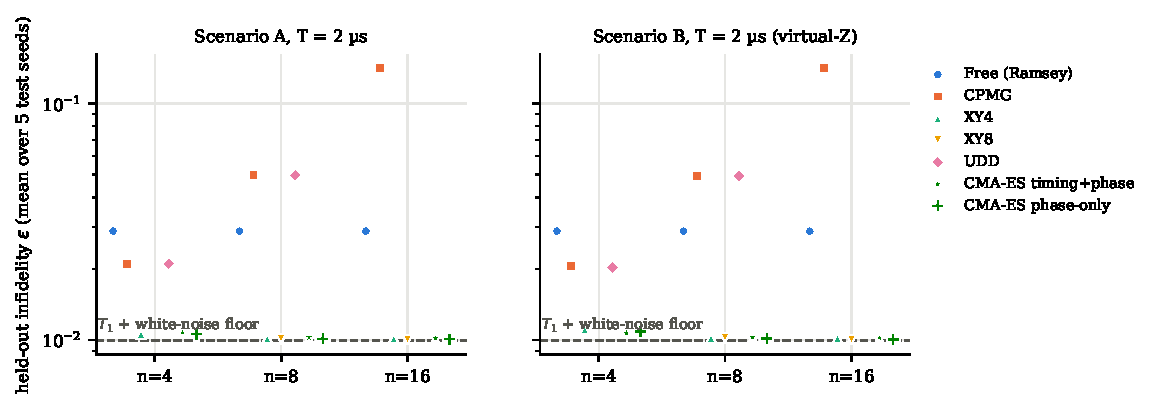
\includegraphics[width=0.92\linewidth]{fig_benchmark.pdf}
\caption{Held-out infidelity of every arm at equal $n$, $T=2\,\mu$s, $w=32$\,ns (mean over test seeds
9001--9005, 1024 trajectories each; CMA-ES: mean over 3 training runs; Monte Carlo standard errors are
smaller than the markers). The dashed line is the analytic floor from $T_1$ and white noise. Scenario~B
arms use virtual-$Z$ from the nominal Stark profile. Near the floor the markers overlap;
Fig.~\ref{fig:benchratio} shows the comparison with the selected baseline as a ratio.}
\label{fig:bench}
\end{figure*}

% >>> BEGIN GENERATED report/generated/bench_table.tex (do not edit; python scripts/manuscript.py sync-generated --write)
\begin{table*}[t]
\centering\scriptsize\setlength{\tabcolsep}{4pt}
\caption{Held-out benchmark at $T=2\,\mu$s, $w=32$\,ns: infidelity $10^3\epsilon$ averaged over test seeds
9001--9005 (1024 trajectories each; MC standard error of each 5-seed mean $\le1.5\%$ of $\epsilon$, per seed $\le3.5\%$). ``Sel.'' = baseline
selected by the pre-registered training-only rule. CMA-ES: mean $\epsilon$ over 3 independent training runs and,
in parentheses, the range of $\epsilon_{\rm sel}/\epsilon_{\rm CMA}$ over runs ($>1$ favours CMA-ES).
Scenario~B arms all use virtual-$Z$ from the nominal Stark profile. UDD-16 is infeasible on the grid
(Table~\ref{tab:feasibility}). Runs: \runid{benchmark\_scenario\_a\_20261026T232517Z\_1bd28ade742a}; \runid{benchmark\_scenario\_b\_20261026T234545Z\_ad7b16de1c23}.}
\label{tab:bench}
\begin{tabular}{@{}lc ccccc c ccc@{}}\toprule
 & & \multicolumn{5}{c}{Canonical baselines} & & \multicolumn{3}{c}{CMA-ES (ratio range)}\\
\cmidrule(lr){3-7}\cmidrule(lr){9-11}
Scenario & $n$ & Free & CPMG & XY4 & XY8 & UDD & Sel. & timing-only & phase-only & timing+phase\\\midrule
A & 4 & 28.8 & 20.9 & 10.6 & --- & 21.0 & XY4 & 21.0 (0.500--0.507) & 10.6 (1.001--1.002) & 10.7 (0.965--1.011) \\
 & 8 & 28.8 & 49.7 & 10.2 & 10.1 & 49.8 & XY8 & 49.8 (0.203--0.203) & 10.1 (0.999--1.000) & 10.2 (0.980--0.992) \\
 & 16 & 28.8 & 141.3 & 10.1 & 10.0 & --- & XY8 & 141.4 (0.071--0.071) & 10.1 (0.996--0.998) & 10.2 (0.982--0.994) \\
\addlinespace
B (virtual-$Z$) & 4 & 28.8 & 20.5 & 11.1 & --- & 20.2 & XY4 & 18.6 (0.568--0.612) & 10.8 (1.008--1.048) & 10.7 (1.024--1.050) \\
 & 8 & 28.8 & 49.2 & 10.2 & 10.2 & 49.3 & XY4 & 41.4 (0.245--0.246) & 10.1 (1.002--1.004) & 10.3 (0.972--1.004) \\
 & 16 & 28.8 & 141.1 & 10.1 & 10.0 & --- & XY8 & 109.6 (0.090--0.093) & 10.1 (0.997--0.999) & 10.2 (0.968--0.993) \\
\bottomrule\end{tabular}\end{table*}
% <<< END GENERATED report/generated/bench_table.tex

\paragraph{Convergence diagnostic} Fig.~\ref{fig:conv} follows a single exploratory training run at
$n=8$ with validation seeds 8001--8002, disjoint from the test seeds. The recorded run contains two
configurations: timing+phase started from CPMG, as in the benchmark, and timing-only with XY8 phases
held fixed. The latter is \emph{not} the pre-registered timing-only arm, which keeps CPMG-$Y$ phases.
Timing+phase training infidelity falls to $\ConvTrainFinal$, below XY8's $\ConvBestBaselineTrain$, while
its validation infidelity stays at $\ConvValFinal$ against $\ConvBestBaselineVal$ for XY8. Timing-only
with XY8 phases reaches $\ConvTimingXYTrainFinal$ (training) and $\ConvTimingXYValFinal$ (validation).
Both training gains come from fitting the 256 frozen trajectories and do not generalize.

\begin{figure}[t]
\centering
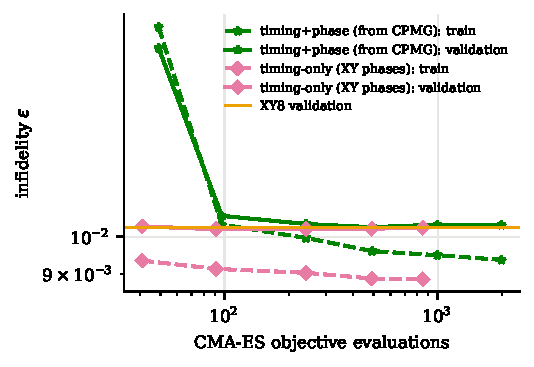
\includegraphics[width=\linewidth]{fig_convergence.pdf}
\caption{Exploratory convergence diagnostic (Scenario~A, $n=8$, training seed 101): training (dashed)
and validation (solid) infidelity of the best-so-far CMA-ES candidate versus evaluations. Green:
timing+phase started from CPMG ($Y$ axes). Pink: timing-only with XY8 phases fixed, a configuration
different from the pre-registered timing-only arm (CPMG-$Y$ phases); its search stopped after 851
evaluations. Horizontal lines: XY8.}
\label{fig:conv}
\end{figure}

\section{Scenario B: robustness (RQ4)}
\label{supp:scenb}
At the nominal Stark profile the bracket formed by the three per-run 95\% Monte Carlo intervals for
$n=4$ timing+phase is $\BenchBFourBothCILo$--$\BenchBFourBothCIHi$; at $n=8,16$ there is no
few-percent gain (Table~\ref{tab:bench}). In the robustness sweep (Table~\ref{tab:robustness},
Fig.~\ref{fig:rob}), $n=4$ timing+phase wins in only $\RobBFourBothWinsMin$--$\RobBFourBothWinsMax$ of
the 10 perturbed profiles (two of which are nominal duplicates), and at $n=8$ two of three runs lose in
all 10. The $n=4$ phase-only sequences remain better than XY4 plus virtual-$Z$ in all 10 perturbations
in all three runs (worst case $\RobBFourPhaseWorstMax$ versus $\RobBFourDDWorst$), a few-percent,
model-specific effect. Virtual-$Z$ alone degrades to $\RobBFourVzWorst$ under a $\pm20\%$ amplitude
error; timing shifts leave it unaffected because the integrated phase of a shift that stays inside the
window is unchanged. No readout-aware sequence design beyond these arms was evaluated.

% >>> BEGIN GENERATED report/generated/robustness_table.tex (do not edit; python scripts/manuscript.py sync-generated --write)
\begin{table}[t]
\centering\scriptsize\setlength{\tabcolsep}{3pt}
\caption{Scenario~B robustness (pre-registered sweep): worst-case $10^3\epsilon$ over 10 perturbed Stark
profiles (amplitude $\times\{0.8,\dots,1.2\}$, timing $\pm\{50,100\}$\,ns and nominal), virtual-$Z$ always from the
nominal profile; CMA-ES values for training runs 101/102/103, and in how many of the 10 perturbations
CMA-ES beats the selected DD + virtual-$Z$. Run \runid{benchmark\_scenario\_b\_20261026T234545Z\_ad7b16de1c23}.}
\label{tab:robustness}
\resizebox{\columnwidth}{!}{\begin{tabular}{@{}clcccc@{}}\toprule
$n$ & CMA-ES mode & VZ only & DD+VZ & CMA-ES+VZ (runs) & wins/10\\\midrule
4 & phase-only & 38.6 & 11.3 (XY4) & 11.2 / 10.6 / 11.2 & 10 / 10 / 10 \\
4 & timing+phase & 38.6 & 11.3 (XY4) & 16.0 / 14.5 / 21.1 & 8 / 6 / 3 \\
8 & phase-only & 38.6 & 10.2 (XY4) & 10.4 / 10.5 / 10.4 & 8 / 8 / 7 \\
8 & timing+phase & 38.6 & 10.2 (XY4) & 10.7 / 19.9 / 20.8 & 9 / 0 / 0 \\
16 & phase-only & 38.6 & 10.0 (XY8) & 10.4 / 10.1 / 10.2 & 0 / 0 / 0 \\
16 & timing+phase & 38.6 & 10.0 (XY8) & 15.0 / 11.2 / 10.5 & 0 / 0 / 0 \\
\bottomrule\end{tabular}}\end{table}
% <<< END GENERATED report/generated/robustness_table.tex

\begin{figure}[t]
\centering
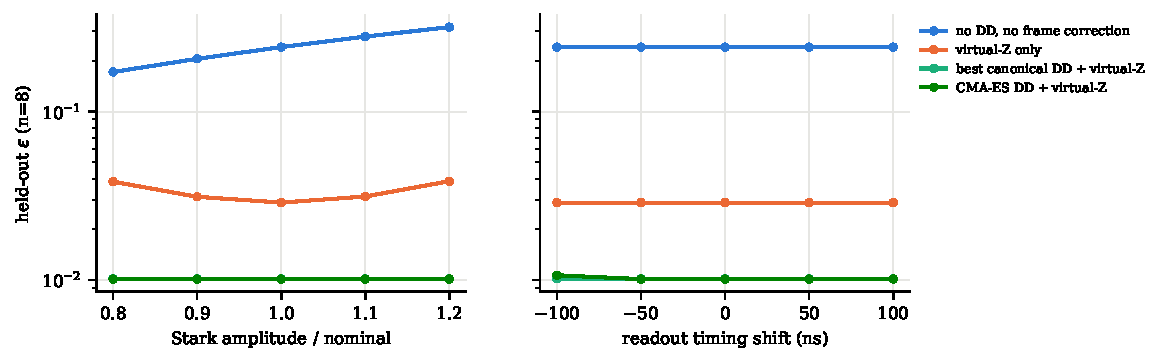
\includegraphics[width=\linewidth]{fig_robustness_b.pdf}
\caption{Scenario~B robustness at $n=4$, all three training runs: (a) Stark amplitude and (b) readout
timing shift perturbed in evaluation while every virtual-$Z$ angle uses the nominal profile.
Timing+phase CMA-ES (dashed) degrades under timing shifts; phase-only (dotted) does not.}
\label{fig:rob}
\end{figure}

\section{Ablations, model mismatch and timing feasibility (RQ5)}
\label{supp:abl}
Table~\ref{tab:ablation} collects the post-hoc ablations. In the colored-only case phase-only gains at
most $\AblColoredFourPhaseRatioHi$ at $n=4$. Within this budget and parameterization (starting from
CPMG, with $2n$ free coordinates) CMA-ES did not find sequences that generalize better than XY-family
designs. The training-only selection rule can pick a baseline that is slightly worse on test (UDD in
the no-amplitude-error ablation), which inflates ratios there by $<1\%$. In the model-based pipeline
(Table~\ref{tab:model_based}) the reduced fitted model gives ratios
$\MBFitRedFourRatioLo$--$\MBFitRedFourRatioHi$ at $n=4$, and its baseline-selection rule sometimes
picks the weaker family. Table~\ref{tab:feasibility} lists the timing constraints of every sequence.

% >>> BEGIN GENERATED report/generated/ablation_table.tex (do not edit; python scripts/manuscript.py sync-generated --write)
\begin{table*}[t]
\centering\scriptsize
\caption{Held-out comparison across scenario variants (test seeds 9001--9005). Ratio
$=\epsilon_{\rm selected}/\epsilon_{\rm CMA}$ (range over 3 training runs; $>1$ favours CMA-ES).
Floor = analytic $T_1$ amplitude damping composed with white dephasing over $T$ (pulse-independent).
$^\dagger$Post-hoc exploratory ablations added after seeing the pre-registered results.}
\label{tab:ablation}
\begin{tabular}{@{}lcccc ccc@{}}\toprule
Variant & $n$ & Sel. & $10^3\epsilon_{\rm sel}$ & $10^3\times$floor & timing-only & phase-only & timing+phase\\\midrule
A (pre-registered), $T=2\,\mu$s & 4 & XY4 & 10.6 & 9.90 & 0.500--0.507 & 1.001--1.002 & 0.965--1.011 \\
 & 8 & XY8 & 10.1 & 9.90 & 0.203--0.203 & 0.999--1.000 & 0.980--0.992 \\
 & 16 & XY8 & 10.0 & 9.90 & 0.071--0.071 & 0.996--0.998 & 0.982--0.994 \\
\addlinespace
A, $T=4\,\mu$s (pre-registered) & 4 & XY4 & 22.8 & 19.6 & 0.693--0.699 & 1.000--1.000 & 0.975--1.003 \\
 & 8 & XY8 & 20.6 & 19.6 & 0.349--0.352 & 0.999--1.000 & 0.939--0.981 \\
 & 16 & XY8 & 19.9 & 19.6 & 0.136--0.136 & 0.997--0.998 & 0.930--0.967 \\
\addlinespace
A without amplitude error$^\dagger$ & 4 & CPMG/UDD & 10.6/10.6 & 9.90 & 0.969--1.007 & 0.999--1.008 & 0.969--1.018 \\
 & 8 & UDD & 10.2 & 9.90 & 0.993--1.007 & 1.007--1.009 & 0.992--1.006 \\
 & 16 & CPMG/XY8 & 10.0/10.0 & 9.90 & 0.987--0.998 & 0.998--0.999 & 0.983--0.997 \\
\addlinespace
A without $T_1$$^\dagger$ & 4 & XY4 & 4.00 & 3.32 & 0.271--0.277 & 1.003--1.004 & 0.917--1.031 \\
 & 8 & XY8 & 3.53 & 3.32 & 0.080--0.081 & 0.996--1.001 & 0.953--1.004 \\
 & 16 & XY8 & 3.45 & 3.32 & 0.025--0.025 & 0.991--0.995 & 0.937--0.994 \\
\addlinespace
A, colored noise only$^\dagger$ & 4 & XY4 & 0.631 & 0.000 & 0.056--0.057 & 1.006--1.010 & 0.967--0.986 \\
 & 8 & XY8 & 0.238 & 0.000 & 0.006--0.006 & 1.002--1.004 & 0.894--0.960 \\
 & 16 & XY8 & 0.098 & 0.000 & 0.001--0.001 & 0.901--0.954 & 0.394--0.566 \\
\bottomrule\end{tabular}\end{table*}
% <<< END GENERATED report/generated/ablation_table.tex
% >>> BEGIN GENERATED report/generated/model_based_table.tex (do not edit; python scripts/manuscript.py sync-generated --write)
\begin{table}[t]
\centering\scriptsize\setlength{\tabcolsep}{3pt}
\caption{Model-based pipeline: baseline selection and CMA-ES (timing+phase) trained on the noise
model in column 1, all arms evaluated on the \textnormal{\emph{true}} Scenario~A model (test seeds 9001--9005).
Fitted models come from run \runid{spectroscopy\_scenario\_a\_20261026T235246Z\_8b272601c344}. Ratio as in Table~\ref{tab:ablation}; CI = envelope of pooled
paired-bootstrap 95\% intervals over the 3 training runs. Run \runid{model\_based\_scenario\_a\_20261026T235628Z\_373dfea37a30}.}
\label{tab:model_based}
\resizebox{\columnwidth}{!}{\begin{tabular}{@{}lcccccc@{}}\toprule
Training model & $n$ & Sel. & $10^3\epsilon_{\rm sel}$ & $10^3\epsilon_{\rm CMA}$ & Ratio & CI envelope\\\midrule
truth & 4 & XY4 & 10.6 & 10.7 & 0.965--1.011 & [0.936, 1.037] \\
fitted full & 4 & XY4 & 10.6 & 10.6 & 0.982--1.011 & [0.960, 1.036] \\
fitted reduced & 4 & XY4 & 10.6 & 11.1 & 0.894--0.984 & [0.873, 1.005] \\
truth & 8 & XY8 & 10.1 & 10.2 & 0.980--0.992 & [0.952, 1.019] \\
fitted full & 8 & XY8 & 10.1 & 10.3 & 0.966--0.991 & [0.927, 1.016] \\
fitted reduced & 8 & XY4/XY8 & 10.1 & 10.7 & 0.896--0.986 & [0.868, 1.011] \\
\bottomrule\end{tabular}}\end{table}
% <<< END GENERATED report/generated/model_based_table.tex
% >>> BEGIN GENERATED report/generated/feasibility_table.tex (do not edit; python scripts/manuscript.py sync-generated --write)
\begin{table}[t]
\centering\scriptsize
\caption{Timing feasibility, square $\pi$ pulses $w=32$\,ns, guard 4\,ns, pulse starts snapped to a
4\,ns grid (assumed controller tick). ``Shift'' = largest change of a pulse centre caused by grid
snapping; ``min gap'' = smallest free gap over feasible families. Infeasible: edge pulses violate the guard after
snapping. Control check: 16$\times$40\,ns pulses in a 500\,ns window is refused by validation.}
\label{tab:feasibility}
\resizebox{\columnwidth}{!}{\begin{tabular}{@{}cclccc@{}}\toprule
$T$ ($\mu$s) & $n$ & Feasible & Infeasible & Max shift (ns) & Min gap (ns)\\\midrule
2 & 4 & CPMG, XY4, UDD & --- & 2.0 & 176 \\
2 & 8 & CPMG, XY4, XY8, UDD & --- & 2.0 & 44 \\
2 & 16 & CPMG, XY4, XY8 & UDD & 1.5 & 48 \\
4 & 4 & CPMG, XY4, UDD & --- & 2.0 & 364 \\
4 & 8 & CPMG, XY4, XY8, UDD & --- & 2.0 & 104 \\
4 & 16 & CPMG, XY4, XY8, UDD & --- & 2.0 & 20 \\
\bottomrule\end{tabular}}\end{table}
% <<< END GENERATED report/generated/feasibility_table.tex

\section{Provenance of the reported runs}
\label{supp:prov}
The dirty-tree runs are listed in the main paper (Sec.~\ref{sec:discussion}); the claim ledger and
its review status are in \repopath{report/evidence\_map.csv}, where every row still awaits human
review. All numbers were regenerated from these checksum-verified runs:\par
{\raggedright\footnotesize\noindent \GenRunIDs.\par}

\end{document}
